\section{Image Elaboration and Feature Extraction}
Once images are acquired and digitized, we can extract important features from them. Usually, we are interested in two primary characteristics:
\begin{itemize}
    \item \textbf{Color} information and its distribution, described by the image's histogram.
    \item \textbf{Shape} information, given by contours and edges of subjects in the image.
\end{itemize}

When dealing with videos, we are also interested in how these features evolve over time. This introduces several challenges:
\begin{itemize}
    \item \textbf{Consistency}: The features of the same object should remain consistent over time, even if the object moves or slightly changes appearance.
    \item \textbf{Evolution}: An object's features can change due to displacements, occlusions, or lighting changes.
    \item \textbf{Scene evolution}: The overall scene can change as new objects appear and old ones disappear.
\end{itemize}

\subsection{Color Analysis: The Histogram}
A histogram is a simple way to describe the color or intensity distribution of an image. It acts as a probability distribution of the pixel values. 
For a grayscale image, the histogram is a 1D array of 256 values, where each bin counts the number of pixels having that specific intensity.

For an $M \times N$ grayscale image $I$:
\begin{itemize}
    \item The sum of all histogram bins equals the total number of pixels:
    \[ \sum_{i=0}^{255} H(i) = M \times N \]
    \item We can normalize the histogram to represent a probability distribution:
    \[ hist(i) = \frac{\text{count}(I(c,r) = i)}{M \times N} \]
\end{itemize}
This concept can be extended to color images by computing a separate histogram for each channel (e.g., R, G, B).

\subsubsection{Information from the Histogram}
The histogram acts as a global signature for the image, providing insights such as:
\begin{itemize}
    \item The \textbf{mean intensity}, indicating if the image is generally bright, dark, or well-exposed.
    \item The \textbf{contrast distribution}, showing whether pixel values are clustered together or spread across the spectrum.
\end{itemize}

\subsubsection{Histogram Operations}
We can manipulate the histogram to enhance the image visually. Various techniques include:

\subsubsection*{Stretching (Contrast Enhancement)}
Stretching improves contrast by expanding the histogram to cover the entire $[0, 255]$ range using a piece-wise linear transformation. 
Given two thresholds, $t_1$ and $t_2$, the transformation from the original pixel intensity $I(c,r)$ to the enhanced intensity $I'(c,r)$ is defined by the following function:

$$I'(c,r) = 
\begin{cases} 
    0 & \text{if } I(c,r) < t_1 \\ 
    \frac{255}{t_2 - t_1} \cdot (I(c,r) - t_1) & \text{if } t_1 \leq I(c,r) \leq t_2 \\ 
    255 & \text{if } I(c,r) > t_2 
\end{cases}$$
The resulting function is piece-wise linear, featuring three distinct segments: a flat segment clamped to 0, a linear mapping segment that scales the intermediate values across $[0, 255]$, and a final flat segment clamped to 255.

\subsubsection*{Equalization}
Ideally, a high-contrast image has a relatively flat histogram where all intensities are equally represented. We can approximate this via \textbf{equalization}:
\begin{itemize}
    \item \textbf{Cumulative Histogram}: First, compute the cumulative distribution:
    \[ CHist_I(i) = \sum_{k=0}^{i} hist(k) \]
    \item \textbf{Transformation}: Then, map the original pixels to new values:
    \[ hist_{equalized}(i) = \frac{CHist_I(i) - CHist_I(0)}{M \times N} \times 255 \]
\end{itemize}

\subsection{Spatial Filtering and Convolution}
To extract shape information or remove noise, we manipulate groups of neighboring pixels. The fundamental mathematical operation used to apply these neighborhood filters is \textbf{convolution}.

\subsubsection{The Convolution Operation}
To apply a filter (often called a kernel or mask) to an image, we perform a 2D convolution between the image $f$ and the filter $h$:
\begin{equation}
    g(x,y) = (f * h)(x,y) = \sum_{i=-\infty}^{\infty} \sum_{j=-\infty}^{\infty} f(i,j) h(x-i, y-j)
\end{equation}
In practical terms, we flip the filter $h$ 180 degrees (equivalent to flipping horizontally and vertically), slide it over the image $f$, and compute the sum of element-wise products at each position.
\begin{figure}[H]
    \centering
    \scalebox{0.8}{
        % filepath: /Users/donny/Documents/GitHub/computer-vision/Tikz/image-videos/convolution.tex

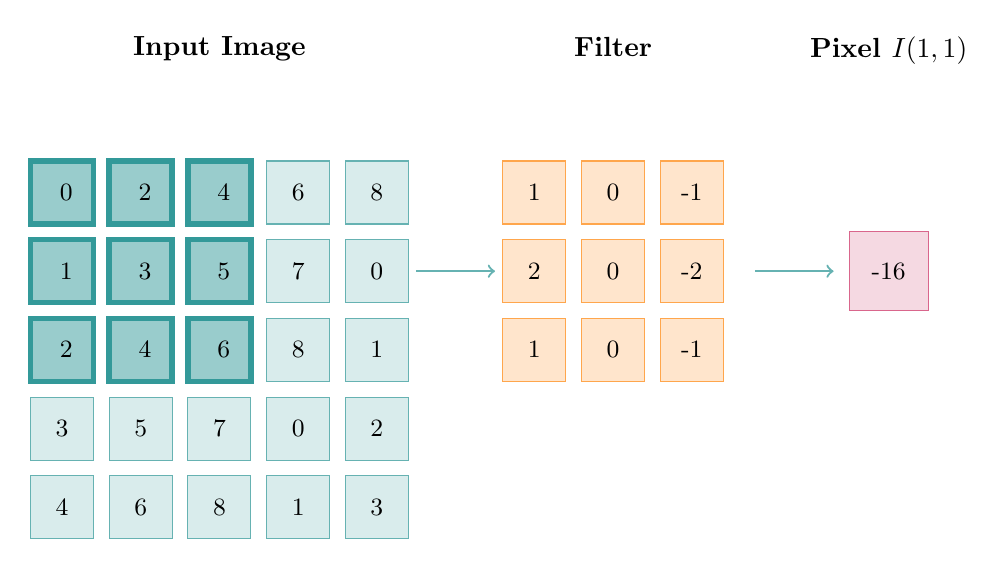
\begin{tikzpicture}[
    cell/.style={draw, rectangle, minimum width=0.8cm, minimum height=0.8cm, font=\small},
    cell-input/.style={cell, fill=teal!15, draw=teal!60},
    cell-highlight/.style={cell, fill=teal!40, draw=teal!80, line width=2pt},
    cell-kernel/.style={cell, fill=orange!20, draw=orange!70},
    cell-output/.style={cell, fill=purple!15, draw=purple!60, minimum width=1cm, minimum height=1cm},
    arrow/.style={->, thick, color=teal!60},
    label/.style={font=\normalsize, font=\bfseries}
]

% --- Input Image Grid (5x5) ---
\node[label, below=0.4cm] at (2, 2.5) {Input Image};
\foreach \i in {0,1,2,3,4} {
    \foreach \j in {0,1,2,3,4} {
        \pgfmathtruncatemacro{\val}{int(mod(\i + 2*\j, 9))}
        \node[cell-input] at (\j,-\i) {\val};
    }
}

% Highlight 3x3 region (top-left 3x3)
\foreach \i in {0,1,2} {
    \foreach \j in {0,1,2} {
        \node[cell-highlight] at (\j,-\i) {
            \pgfmathtruncatemacro{\val}{int(mod(\i + 2*\j, 9))}
            \val
        };
    }
}

% --- Kernel (3x3) ---
\node[label, below=0.4cm] at (7, 2.5) {Filter};
\node[cell-kernel] at (6, 0) {1};
\node[cell-kernel] at (7, 0) {0};
\node[cell-kernel] at (8, 0) {-1};

\node[cell-kernel] at (6, -1) {2};
\node[cell-kernel] at (7, -1) {0};
\node[cell-kernel] at (8, -1) {-2};

\node[cell-kernel] at (6, -2) {1};
\node[cell-kernel] at (7, -2) {0};
\node[cell-kernel] at (8, -2) {-1};

% --- Arrow ---
\draw[arrow] (4.5,-1) -- (5.5,-1);
\draw[arrow] (8.8,-1) -- (9.8,-1);
% --- Output ---
\node[label, below=0.4cm] at (10.5, 2.5) {Pixel $I(1,1)$};
\node[cell-output] at (10.5, -1) {-16};

\end{tikzpicture}
    }
    \caption{Example of convolution between an image and a filter.}
\end{figure} 
\textit{Note:} The output must be stored in a separate, new image array to ensure we process subsequent pixels using the original, unmodified neighboring values.

\subsubsection*{Handling image borders}
When the filter overlaps the borders of the image, we cannot compute the convolution as usual, since some neighboring pixels are missing.
Common strategies to handle this include:
\begin{itemize}
    \item \textbf{Zero-padding}: Assume missing pixels are 0.
    \item \textbf{Replication}: Replicate the nearest border pixel values.
    \item \textbf{Reflection}: Mirror the image across the border.
\end{itemize}

\subsubsection{Smoothing and Enhancement (Low-pass Filters)}
Smoothing removes high-frequency components (like sharp edges and noise), leaving behind low-frequency components (smooth regions).
We will now discuss three common low-pass filters: the average filter, the Gaussian filter, and the median filter.

\subsubsection*{Average Filter}
A simple average filter uses a kernel of size $k \times k$ (e.g., $5 \times 5$) where each element is $\frac{1}{k^2}$. 
The output pixel value is the average of the neighboring pixels. For a $5 \times 5$ kernel, the output pixel at position $(c,r)$ is computed as:
\begin{equation}
    I'(c,r) = \frac{1}{25} \sum_{i=-2}^{2} \sum_{j=-2}^{2} I(c+i, r+j)
\end{equation}
The larger the kernel, the stronger the blur. 

\subsubsection*{Gaussian Filter}
A Gaussian filter is a weighted low-pass filter that uses a kernel defined by the two-dimensional Gaussian function, 
which is typically centered at the origin of the kernel:

\begin{equation}
    G(x,y) = c e^{-\frac{x^2 + y^2}{2\sigma^2}}
\end{equation}
where $x$ and $y$ represent the displacement from the center of the kernel. The variable $\sigma$ controls the spread of the Gaussian, and $c$ is a normalization constant ensuring that the sum of all kernel values equals 1. 

Unlike a simple average filter, it assigns higher importance to pixels that are closer to the center of the kernel, resulting in a more natural and visually pleasing blur.
It is \textbf{isotropic} (circularly symmetric), meaning it smooths equally in all directions. The standard deviation $\sigma$ controls the blur intensity.

\subsubsection*{Median Filter}
Unlike convolution-based filters, the median filter is non-linear. 
It sorts the neighborhood pixels by value and outputs the statistical median. 
It is highly robust to outliers and is particularly effective at removing "salt-and-pepper" (spike) noise without heavily blurring edges.

\subsubsection{Edge Detection (High-Pass Filtering)}

Edges represent abrupt spatial variations in image intensity and are fundamental features for image analysis. Detecting edges requires estimating local intensity variations, which can be achieved through image derivatives.

\subsubsection*{Gradient-Based Edge Detection}
Since images are defined over a two-dimensional domain, intensity changes must be analyzed along both the horizontal ($x$) and vertical ($y$) directions. Let $f(x,y)$ denote the image intensity function. The rate of change along a generic direction $r$, identified by an angle $\theta$, is given by the directional derivative:
\begin{equation}
    \frac{\partial f}{\partial r}
    =
    f_x \cos\theta + f_y \sin\theta
\end{equation}
where $f_x$ and $f_y$ denote the partial derivatives of the image intensity with respect to $x$ and $y$, respectively.

The \textbf{direction} of maximum intensity variation corresponds to the gradient orientation, obtained by maximizing the directional derivative with respect to $\theta$:
\begin{equation}
    \theta_g
    =
    \tan^{-1}\left(\frac{f_y}{f_x}\right)
\end{equation}

The \textbf{strength} of the edge is quantified by the gradient magnitude:
\begin{equation}
    \|\nabla f\|
    =
    \sqrt{f_x^2 + f_y^2}
\end{equation}

\subsubsection*{Discrete Gradient Approximation: Sobel Filters}
In practical image processing applications, continuous derivatives are approximated using discrete convolution kernels. 
A common choice is the \textbf{Sobel operator}, which estimates image gradients along the horizontal and vertical directions through finite impulse response (FIR) filters:
\begin{equation}
    G_x =
    \begin{bmatrix}
    -1 & 0 & 1 \\
    -2 & 0 & 2 \\
    -1 & 0 & 1
    \end{bmatrix},
    \qquad
    G_y =
    \begin{bmatrix}
    -1 & -2 & -1 \\
    0 & 0 & 0 \\
    1 & 2 & 1
    \end{bmatrix}
\end{equation}

After convolving the image with these kernels, the horizontal and vertical responses, denoted as $D_x$ and $D_y$, are combined to estimate the overall edge intensity:
\begin{equation}
    D
    =
    \sqrt{D_x^2 + D_y^2}
\end{equation}
\subsubsection*{Binarization}
Once we compute the continuous edge strengths, we apply a threshold to create a binary image: pixels above the threshold are classified as "edge" (1), and those below as "background" (0).

\subsection{Morphological Filters}
Morphology operators are non-linear transformations typically applied to \textbf{binary images} (like those produced after edge binarization). They use a \textbf{Binary Structuring Element} (BSE) to analyze, extract, or fit shapes within the image.

\subsubsection{Fundamental Operations}
\begin{itemize}
    \item \textbf{Dilation}: The structuring element $S$ is swept over the binary image $B$. If the origin of $S$ touches a foreground pixel (1), all pixels covered by $S$ are set to 1. This expands shapes and bridges small gaps.
    \begin{equation}
        B \oplus S = \bigcup_{b \in B} S_b
    \end{equation}
    \item \textbf{Erosion}: The structuring element $S$ is swept over $B$. A pixel remains 1 only if the \textit{entire} structuring element fits completely inside the foreground. This shrinks shapes and removes small isolated noise.
\end{itemize}

\subsubsection{Compound Operations}
Opening and closing are combinations designed to clean up shapes without drastically changing their overall area:
\begin{itemize}
    \item \textbf{Opening (Erosion followed by Dilation)}: Removes small objects or thin protrusions from the foreground while preserving the size of larger shapes.
    \item \textbf{Closing (Dilation followed by Erosion)}: Fills small holes and smooths inward-curving boundaries without expanding the overall shape.
\end{itemize}